\documentclass{article}

\usepackage{amsmath,amssymb}
\usepackage{geometry}
\usepackage{graphicx}

\geometry{a4paper, margin=2.5cm}

\begin{document}

% ============================================================
\section*{Actor-Critic and A2C}

\subsection*{First, a story}

You are learning the piano. Your teacher has two ways of teaching.

\textbf{Method 1 (REINFORCE)}: you play the whole piece; the teacher grades at the end --- ``85 overall''. Can that single number tell you which note was wrong? No. The chord that slipped in bar 3 and the tempo that ran away in bar 12 all drown in the single ``85''. You can only guess your way to improvement.

\textbf{Method 2 (Actor-Critic)}: the teacher sits beside you, offering a comment every few notes --- ``too fast here'', ``that chord is wrong'', ``nicely phrased''. Immediate, localized feedback; progress is much faster.

But a new problem appears: if, after three notes, the teacher decides ``I've got this student's level all figured out'', stops listening carefully and just says ``fine'' from then on --- from that moment your practice loses its feedback and progress stops dead.

\textbf{That is the essence of naive Actor-Critic's failure} --- not a wrong direction, but the policy collapsing prematurely (without entropy protection) into a deterministic one, after which the critic fits the value of this \underline{very poor} policy nearly perfectly, the advantage signal goes to zero, and the actor's gradient vanishes.

The core problem of this chapter: \textbf{how do we keep the critic's learning rate matched to the actor's pace of improvement?}

\subsection*{From REINFORCE to Actor-Critic: why replace the return}

REINFORCE's policy-gradient estimator:

\[
\nabla_\theta J(\theta) = \mathbb{E}_{\tau \sim \pi_\theta}\!\left[\,\sum_{t=0}^{T}
\nabla_\theta \log \pi_\theta(a_t \mid s_t) \cdot G_t\,\right]
\]

with $G_t = \sum_{k=t}^{T} \gamma^{k-t} r_k$ the discounted reward from step $t$ to the end (the Monte Carlo return).

\textbf{Where the high variance comes from}: $G_t$ depends on all future random actions and rewards after $t$. The longer the episode, the noisier $G_t$ --- judging ``was the fingering in bar 3 right'' by ``the final grade of the whole piece'' has a terrible signal-to-noise ratio.

\textbf{The core substitution}: let $V^\pi(s)$ provide a baseline, replacing $G_t$ by ``how much better than average'':

\[
\boxed{G_t \;\longrightarrow\; A^\pi(s_t, a_t) = Q^\pi(s_t, a_t) - V^\pi(s_t)}
\]

This is the \textbf{advantage function}. $A > 0$ means ``this action is better than average''; $A < 0$ means ``worse''. Two benefits: (1) subtracting the action-independent baseline $V$ cuts variance; (2) it measures relative quality, sharpening the signal.

% ============================================================
\section*{The Advantage Function and the TD Error}

\subsection*{Formalization}

Let the current policy be $\pi_\theta$ and the parameterized value be $V_\phi(s)$:

\begin{itemize}
  \item \textbf{State value}: $V^\pi(s) = \mathbb{E}_\pi\!\left[\sum_{k=0}^{\infty} \gamma^k r_{t+k} \,\Big|\, s_t=s\right]$
  \item \textbf{Action value}: $Q^\pi(s,a) = \mathbb{E}_\pi\!\left[\sum_{k=0}^{\infty} \gamma^k r_{t+k} \,\Big|\, s_t=s,\,a_t=a\right]$
  \item \textbf{Advantage}: $A^\pi(s,a) = Q^\pi(s,a) - V^\pi(s)$
\end{itemize}

Note $\mathbb{E}_{a \sim \pi}\!\left[A^\pi(s,a)\right] = 0$ --- the advantage has zero mean by construction: good and bad actions sit symmetrically on either side of zero.

\subsection*{The one-step TD error as an advantage estimate}

Computing the true $Q^\pi(s,a)$ needs the full future reward sequence. A feasible approximation:

\[
Q^\pi(s_t, a_t) \approx r_t + \gamma V^\pi(s_{t+1}) \quad \text{(one-step bootstrap)}
\]

Substituting into the advantage definition gives the \textbf{one-step TD error}:

\[
\boxed{\delta_t = r_t + \gamma V_\phi(s_{t+1}) - V_\phi(s_t)}
\]

\textbf{In plain words}: $\delta_t$ is ``the reward actually received plus the new expectation of the future'' minus ``the old expectation at departure''. More $\Rightarrow$ this action beat expectations (positive advantage); less $\Rightarrow$ below (negative).

\textbf{Where the bias comes from}: $\delta_t$ replaces the true $V^\pi$ with the approximate $V_\phi$, adding function-approximation error (bias). That is the essential trade-off against Monte Carlo: \textbf{lower variance, but no longer unbiased}.

% ============================================================
\section*{Why naive Actor-Critic fails}

\subsection*{Four fault modes}

The most direct implementation: replace REINFORCE's per-episode update with per-step online updates and $G_t$ with $\delta_t$. The idea is right, but four latent problems lurk:

\begin{enumerate}
  \item \textbf{Fault 1 --- one-step TD advantage, variance still high}\\
        $\delta_t$ looks only one step ahead, buffeted by both random rewards and $V_\phi$'s estimation error. Before $V_\phi$ converges, $\delta_t$ is extremely unstable and the actor's gradient is noisy.

  \item \textbf{Fault 2 --- the two-timescale condition is violated}\\
        Konda \& Tsitsiklis (2003) proved: Actor-Critic convergence requires the critic's learning rate $\alpha_w$ to be much larger than the actor's $\alpha_\theta$, i.e.\ $\alpha_\theta / \alpha_w \to 0$. Naive implementations use one learning rate for both, so the actor updates before the critic has converged, computing gradient directions from a wrong $V_\phi$.

  \item \textbf{Fault 3 --- no entropy regularization, premature collapse}\\
        Without an entropy bonus the actor piles probability onto some suboptimal action and becomes near-deterministic. Once the action distribution has no randomness, the policy gradient cannot drive exploration even when $\delta_t$ is occasionally nonzero.

  \item \textbf{Fault 4 --- no gradient clipping, parameters can explode}\\
        Single-step $|\delta_t|$ is occasionally huge (badly initialized $V_\phi$), causing enormous updates that push the network into unrecoverable regions.
\end{enumerate}

\subsection*{The collapse mechanism: advantage vanishing $\Rightarrow$ actor freezes}

Once Fault 3 triggers, the four faults couple into a self-reinforcing loop:

\[
\text{no entropy} \;\Rightarrow\; \pi \text{ becomes deterministic rapidly}
\;\Rightarrow\; \text{every episode degenerates into the same short trajectory}
\]
\[
\Rightarrow\; V_\phi \text{ fits those trajectories quickly (} \delta_t \approx 0 \text{)}
\;\Rightarrow\; \nabla_\theta J \approx 0 \;\Rightarrow\; \text{the actor freezes forever.}
\]

This is a \textbf{stable but catastrophic fixed point}: the more ``perfect'' the critic, the less incentive the actor has to move; the more the actor freezes, the more solid the critic. The system locks itself in --- almost identically across seeds.

\subsection*{Experimental evidence}

Figure~\ref{fig:naive} shows naive Actor-Critic on CartPole-v1 across 5 seeds: the return pins at $\approx 9$ (CartPole-v1's maximum is 500) from about episode 20, with zero progress over 500 episodes. The five curves nearly overlap --- not randomness but the same bad fixed point in every seed.

\begin{figure}[!htbp]
  \centering
  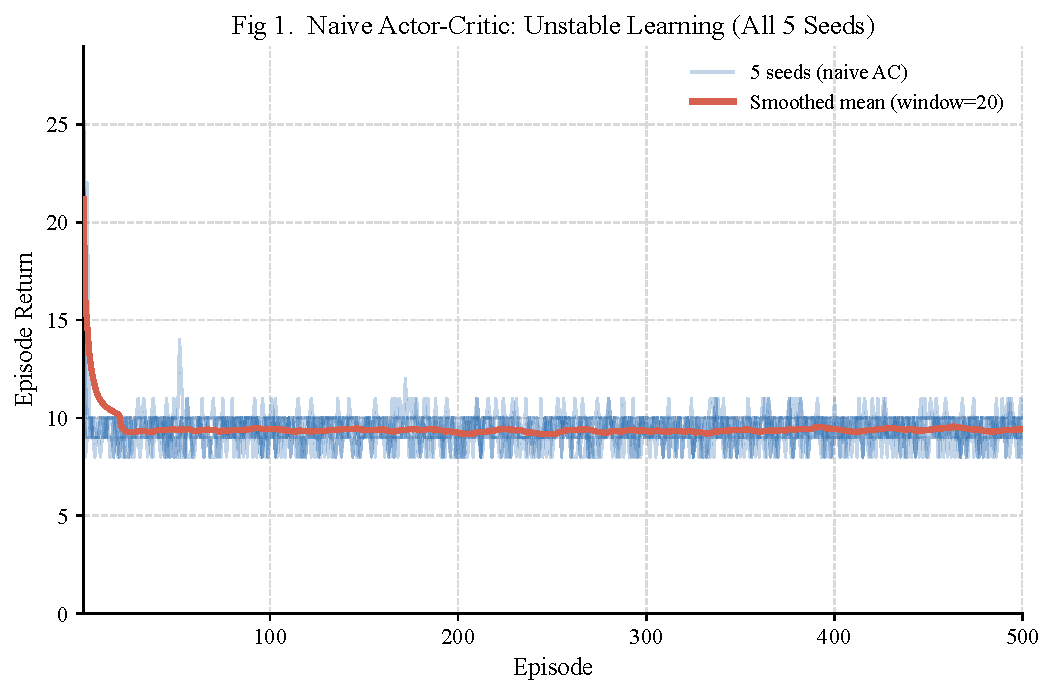
\includegraphics[width=\textwidth]{fig1_naive_ac_failure.pdf}
  \caption{Naive Actor-Critic ($\alpha = 5 \times 10^{-3}$, no entropy, no gradient clipping) on CartPole-v1, 5 random seeds: the return is pinned at $\approx 9$ throughout; the maximum return of CartPole-v1 is 500.}
  \label{fig:naive}
\end{figure}

Figure~\ref{fig:adv} gives direct evidence of the collapse: the mean $|\text{advantage}|$ of naive AC plummets from $\approx 3.5$ to $\approx 0.1$ within the first 50 episodes and hugs zero thereafter --- the actor's gradient signal has vanished. In contrast, A2C's $|\text{advantage}|$ traces a \textbf{bell curve} --- rising as the policy improves (the critic cannot keep up), then smoothly falling as convergence nears --- the healthy signature of an online learning system.

\begin{figure}[!htbp]
  \centering
  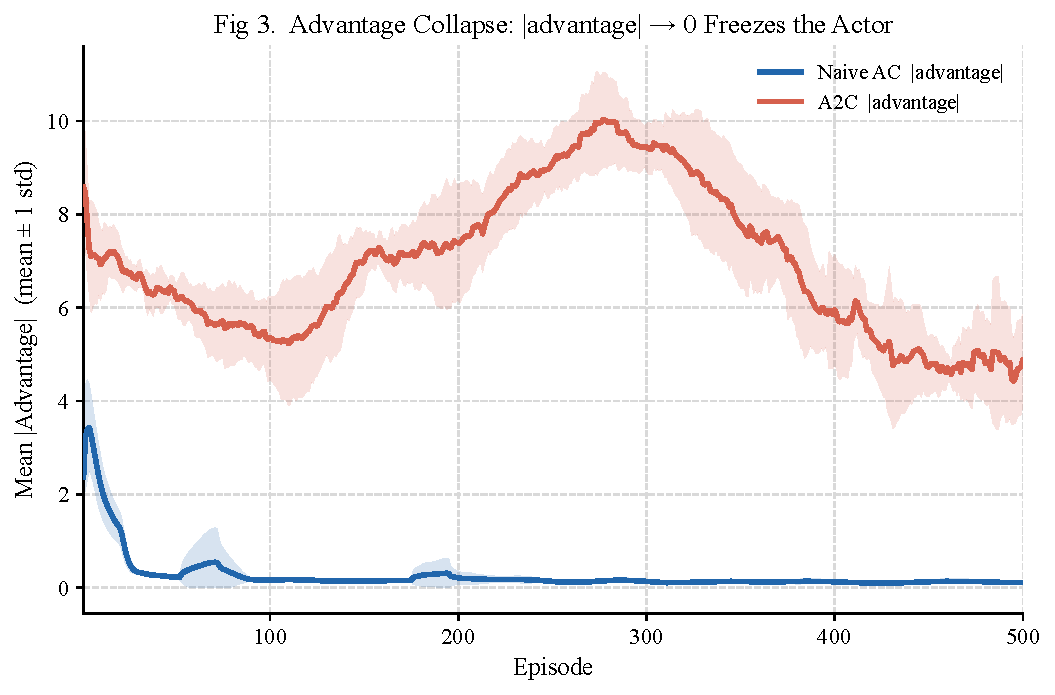
\includegraphics[width=\textwidth]{fig3_advantage_collapse.pdf}
  \caption{Mean per-episode $|\hat{A}_t|$ (5 seeds, mean $\pm$ 1 std). Blue (naive AC) hits zero within 50 episodes; red (A2C) maintains nonzero signal with a bell shape reflecting the persistent catch-up dynamics between critic and actor.}
  \label{fig:adv}
\end{figure}

% ============================================================
\section*{Generalized Advantage Estimation (GAE)}

\subsection*{The mathematical frame of the bias--variance trade-off}

The one-step TD error $\delta_t$ is high-bias (when $V_\phi$ is inaccurate); the Monte Carlo return $G_t - V(s_t)$ is high-variance (longer trajectories, more randomness). Can we find a tunable middle point?

Schulman et al.\ (2015) proposed the \textbf{Generalized Advantage Estimator (GAE)}:

\[
\boxed{\hat{A}_t^{\,\text{GAE}(\gamma,\lambda)} = \sum_{l=0}^{\infty} (\gamma\lambda)^l \,\delta_{t+l}}
\]

Each $\delta_{t+l} = r_{t+l} + \gamma V(s_{t+l+1}) - V(s_{t+l})$ is the TD error at step $t+l$, with $\lambda \in [0,1]$ the interpolation parameter.

\subsection*{Derivation: GAE as a geometric series of TD errors}

Expanding the first $n$ terms:

\[
\hat{A}_t^{(n)} = \sum_{l=0}^{n-1} (\gamma\lambda)^l \delta_{t+l}
= \delta_t + \gamma\lambda\,\delta_{t+1} + (\gamma\lambda)^2 \delta_{t+2} + \cdots
\]

The two extremes:

\begin{itemize}
  \item $\lambda = 0$: $\hat{A}_t = \delta_t$ (one-step TD), \textbf{high bias, low variance}, entirely dependent on $V_\phi$'s accuracy;
  \item $\lambda = 1$: $(\gamma\lambda)^l = \gamma^l$, summing all future TD errors; telescoping gives
\end{itemize}

\[
\hat{A}_t^{\lambda=1} = \sum_{l=0}^{T-t-1}\gamma^l \delta_{t+l}
= \underbrace{\sum_{l=0}^{T-t-1}\gamma^l r_{t+l}}_{G_t} - V(s_t) + \gamma^{T-t}V(s_T)
\approx G_t - V(s_t), \quad \text{(terminal }V(s_T)\approx 0\text{)}
\]

i.e.\ REINFORCE's baseline advantage: \textbf{low bias, high variance}.

\[
\begin{array}{c|c|c}
\lambda & \text{extreme case} & \text{bias / variance} \\
\hline
0 & \hat{A}_t = \delta_t \;\text{(one-step TD)} & \text{high bias, low variance} \\
1 & \hat{A}_t = G_t - V(s_t) \;\text{(Monte Carlo)} & \text{low bias, high variance} \\
\lambda \in (0,1) & \text{geometric interpolation} & \text{tunable trade-off} \\
\end{array}
\]

\textbf{Why geometric decay is sensible}: near-term TD errors have a higher signal-to-noise ratio ($V_\phi$ predicts near states better); distant ones accumulate more randomness. Weighting the near term more via $(\gamma\lambda)^l$ is an implicit exponential smoothing of the gradient estimate.

\subsection*{Using GAE in practice}

GAE needs the full sequence of TD errors, so finish a whole rollout first, then recurse backwards from the end:

\[
\hat{A}_{T-1} = \delta_{T-1}, \qquad
\hat{A}_t = \delta_t + \gamma\lambda\,\hat{A}_{t+1} \quad (t = T-2, \ldots, 0)
\]

The corresponding \textbf{critic target} (the return estimate):

\[
\hat{R}_t = \hat{A}_t + V_\phi(s_t)
\]

\textbf{Choosing $\lambda$}: $\lambda = 0.95$ is the empirical default, working well on most continuous and discrete control tasks (Schulman et al.\ 2015, 2017).

% ============================================================
\section*{Advantage Actor-Critic (A2C): four fixes}

\subsection*{Patching the four faults one by one}

\begin{enumerate}
  \item \textbf{Fix 1 --- full-episode rollout $+$ GAE}\\
        Collect a complete trajectory before computing all advantages, replacing one-step $\delta_t$ by GAE ($\lambda = 0.95$): lower variance than one-step TD, lower bias than Monte Carlo.

  \item \textbf{Fix 2 --- two-timescale learning rates}\\
        Critic learning rate $\alpha_w = 10^{-3}$, actor $\alpha_\theta = 3\times 10^{-4}$ ($\alpha_w / \alpha_\theta \approx 3$). The critic learns faster each round, so the actor's next update uses a more accurate $V_\phi$.

  \item \textbf{Fix 3 --- entropy regularization}\\
        Add an entropy term to the actor loss to prevent premature collapse to a deterministic distribution:
        \[
        L_{\text{actor}} = -\hat{A}_t \log\pi_\theta(a_t \mid s_t) - \beta\,\mathcal{H}[\pi_\theta(\cdot \mid s_t)], \quad \beta = 0.01
        \]

  \item \textbf{Fix 4 --- gradient clipping}\\
        Clip gradients by max-norm before stepping (clip $= 0.5$), preventing one oversized update from blowing up the parameters.
\end{enumerate}

\subsection*{The full algorithm}

\begin{enumerate}
  \item \textbf{Rollout (no gradients)}: run one episode with the current $\pi_\theta$ and $V_\phi$, recording $(s_t,a_t,r_t,V_\phi(s_t))_{t=0}^{T}$;
  \item \textbf{Compute GAE advantages}: recurse backwards from the end; compute return targets $\hat{R}_t = \hat{A}_t + V_\phi(s_t)$;
  \item \textbf{Normalize advantages}: $\hat{A}_t \leftarrow (\hat{A}_t - \bar{A}) / (\sigma_A + \varepsilon)$, stabilizing gradient magnitudes;
  \item \textbf{Critic update (higher learning rate)}:
        \[
        L_{\text{critic}} = \frac{1}{2}\left\|\,V_\phi(s_t) - \hat{R}_t\,\right\|^2,
        \quad \text{step with } \alpha_w \text{ after gradient clipping;}
        \]
  \item \textbf{Actor update (lower learning rate)}:
        \[
        L_{\text{actor}} = -\hat{A}_t\log\pi_\theta(a_t \mid s_t) - \beta\,\mathcal{H}[\pi_\theta(\cdot\mid s_t)],
        \quad \text{step with } \alpha_\theta \text{ after gradient clipping.}
        \]
\end{enumerate}

\subsection*{Results}

Figure~\ref{fig:compare} shows 5-seed mean $\pm$ 1 std curves: A2C rises steadily from about episode 50, reaching a mean of $\approx 310$ at episode 500 while still climbing (not fully converged); naive AC hugs the $x$ axis; the two separate completely after episode 50.

\begin{figure}[!htbp]
  \centering
  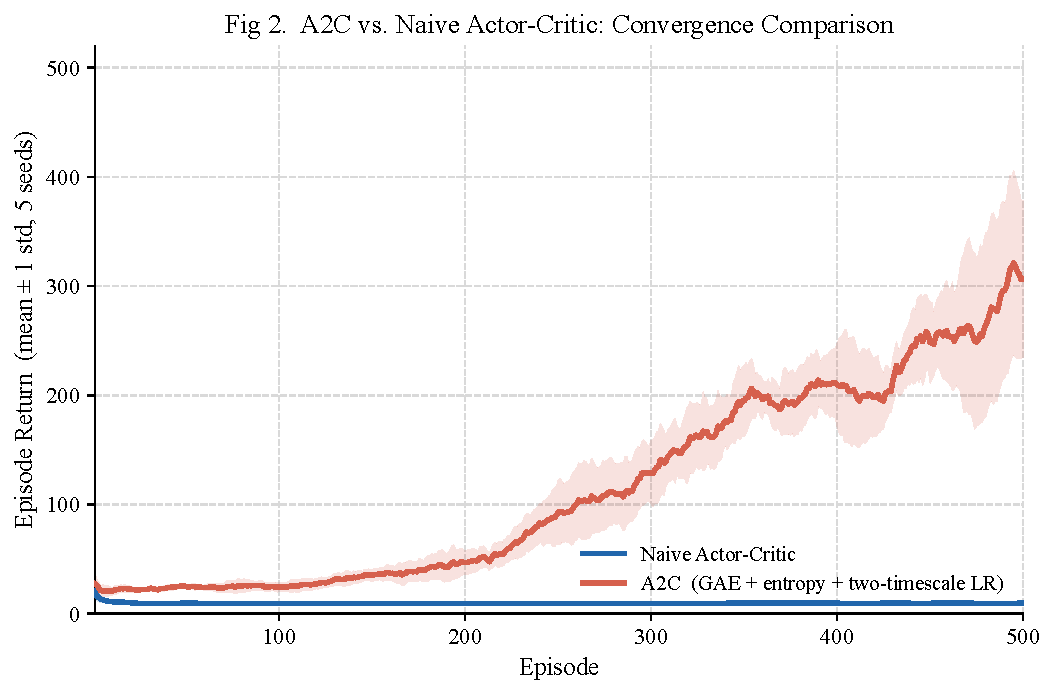
\includegraphics[width=\textwidth]{fig2_a2c_vs_naive.pdf}
  \caption{A2C vs.\ naive Actor-Critic on CartPole-v1 (5 seeds, mean $\pm$ 1 std, identical network architecture; only training differs).}
  \label{fig:compare}
\end{figure}

Revisit Figure~\ref{fig:adv}'s A2C curve (the red bell): the advantage keeps growing for the first $\sim 280$ episodes --- the phase of fast return growth in Figure~\ref{fig:compare}, where the policy improves faster than the critic can track; afterwards it falls smoothly as the critic catches up and the return curve's slope eases. \textbf{The critic--actor catch-up dynamic is exactly the healthy state the two-timescale design wants to maintain.}

% ============================================================
\section*{Algorithm comparison}

\[
\begin{array}{c|c|c|c}
\text{Method} & \text{Advantage estimate} & \text{Update timing} & \text{Bias / variance} \\
\hline
\text{REINFORCE} & G_t & \text{end of episode} & \text{low bias, very high variance} \\
\text{REINFORCE + Baseline} & G_t - V(s_t) & \text{end of episode} & \text{low bias, high variance (improved)} \\
\text{naive AC} & \delta_t & \text{online, per step} & \text{high bias, low variance (but collapses)} \\
\text{A2C} & \hat{A}^{\text{GAE}(\gamma,\lambda)} & \text{batched after episode} & \text{tunable via } \lambda\text{, stable} \\
\end{array}
\]

\subsection*{Why not just use Monte Carlo returns in A2C?}

Using pure MC returns $G_t$ as the critic target reduces A2C to REINFORCE with baseline --- bootstrap's variance advantage disappears. On \textbf{short-episode} tasks like CartPole-v1 MC is usable, but on continuous-control (high-dimensional action spaces such as joint angles and velocities) plus long episodes, $G_t$'s variance becomes unmanageable. GAE's $\lambda$ interpolates continuously over the bias--variance trade-off instead of choosing one extreme.

\subsection*{Why should the critic's learning rate exceed the actor's?}

\textbf{The two-timescale theorem} (Konda \& Tsitsiklis 2003): Actor-Critic convergence requires

\[
\sum_k \alpha_\theta(k) = \infty, \quad \sum_k \alpha_w(k) = \infty, \quad
\frac{\alpha_\theta(k)}{\alpha_w(k)} \to 0 \quad (k \to \infty)
\]

\textbf{Intuition}: if actor and critic move at the same speed, the critic forever chases a moving target (the policy keeps changing). A faster critic approximately converges to the current policy's $V^\pi$ before the actor's next update, guaranteeing the actor a ``trustworthy evaluation of the current policy'' --- gradient directions it can trust.

% ============================================================
\section*{Where this chapter sits in the RL landscape}

Actor-Critic is the bridge from basic algorithms to modern deep RL:

\begin{enumerate}
  \item \textbf{The TD route (value-based)}: MAB $\to$ MDP / Bellman equations $\to$ TD(0) / Q-Learning $\to$ DQN. DQN learns $Q(s,a)$ --- a pure critic with no explicit actor; it cannot handle continuous action spaces.

  \item \textbf{The MC route (policy-based)}: REINFORCE optimizes $\pi_\theta$ directly --- a pure actor with no critic; enormous variance, low sample efficiency.

  \item \textbf{The Actor-Critic route (fusion)}: this chapter merges the two --- the actor optimizes the policy while the critic supplies a low-variance baseline. GAE tunes the bias--variance trade-off $\to$ \textbf{PPO} (next chapter) adds a clip constraint on the AC framework to bound each policy update $\to$ \textbf{SAC} pushes entropy regularization to a firmer theoretical footing with automatic temperature tuning.

  \item \textbf{The shadow of offline RL}: in offline methods such as IQL (Implicit Q-Learning) the critic still needs accurate value estimates; the two-timescale principle reappears in another guise --- \underline{how to keep the critic from overfitting out-of-distribution states when coverage is thin} is precisely the question offline RL answers.
\end{enumerate}

Remove PPO's clip objective, keeping GAE + entropy + gradient clipping --- how different is what remains from this chapter's A2C? What exactly does PPO's clip prevent?

\subsection*{References}

\begin{enumerate}
  \item Konda \& Tsitsiklis (2003). On actor-critic algorithms. \textit{SIAM Journal on Control and Optimization}, 42(4).
  \item Sutton \& Barto (2018). \textit{Reinforcement Learning: An Introduction} (2nd ed.). Chapter 13.
  \item Schulman et al.\ (2015). High-dimensional continuous control using generalized advantage estimation. \textit{ICLR 2016}.
  \item Mnih et al.\ (2016). Asynchronous methods for deep reinforcement learning (A3C). \textit{ICML}.
  \item Hands-on RL (Chinese). Chapter 12: Actor-Critic algorithms.
\end{enumerate}

\end{document}
